\documentclass[10pt,a4paper]{article}
\usepackage[utf8]{inputenc}
\usepackage{amsmath}
\usepackage{amsfonts}
\usepackage{amssymb}
\usepackage{graphicx}
\usepackage{hyperref}
\usepackage[margin=1in]{geometry}


\author{Jessica Chemali, Kumar Shaurya Shankar, Trenton Tabor\\kumarsha@cs.cmu.edu}
\title{16831 RoboStats Lab 2: \\Online Learning}
\begin{document}
\maketitle
\section{Overview}
\subsection{Discussion about Dataset}
Mention balancing of data here
Mention Shuffling of data here

We implemented k-fold cross validation to tune our parameters.

Some classes are easily distinguishable but others like wire/pole are not.
%----------------------------------------------------------------------
\section{Implemented methods}
\subsection{Bayes Linear Regression}
\subsubsection{Implementation}
The Bayes Linear Regressor has been implemented in Python, as the rest of the framework. The external library dependency is only on numpy for matrix operations and normal distribution functions. The algorithm has not been modified for the purpose of this implementation.
\subsubsection{Parameter Selection}
The three parameter choices are the initial natural parameters for the prior on the weight vector, and the noise variance for the observation error. The latter was arbitrarily chosen, but **TODO*** should be cross validated. For the prior, a 0 mean weight vector was chosen, and a unit precision matrix was chosen. ***TODO**** can I provide better priors looking at data, for instance covariance of data?
\subsubsection{Performance}
figure

\subsubsection{Learning Duration}
Learning is very fast since this is linear regression. ***TODO*** Timing?

\subsubsection{Robustness to Noise}
****TODO*** Don't expect to be too robust.
%------------------------------------------------------------------------
\subsection{Multiclass exponentiated gradient algorithm}

\subsubsection{Winnow with binary features}
We first implemented Winnow algorithm with binary features, after discretizing every feature based on the resulting entropy of the partition. It gave terrible results, because it turned out that the binary features weren't informative enough to differentiate well between the classes and the performance of the algorithm depended tremendously on the order the observations were presented to the algorithm. 

\subsubsection{Generalization of winnow to continuous features}

The algorithm that we will discuss is similar to winnow but instead, when the algorithm makes a mistake, it updates the weight of feature $i$ using the equation : $w_i = w_i*exp(\nu x_i y_i)$. 

Trainig online was affected considerably by the order the data was presented to the algorithm. This is why we shuffled the data before training the algorithm and in this way reached better results.

Training on the "an" dataset was easier and resulted in around $90\%$ accuracy on the heldout "am" dataset. The confusion matrix, which is more useful showed that thhe algoithm predicted very well class $1200$ with very little negatives, followed by class $1004$, and class $1400$. Classes $1100$ and $1103$, corresponding to the poles and wires were poorly learned.

Training on the "an" dataset and testing on the heldout "am" dataset was easier than the other way around and resulted in an accuracy of around $90\%$ versus an accuracy of $70\%$ on the heldout datasets. The confusion matrix, which is more useful showed that thhe algoithm predicted very well class $1200$ with very little negatives, followed by class $1004$, and class $1400$. Classes $1100$ and $1103$, corresponding to the poles and wires were poorly learned. This is not surprising because the datasets were highly unbalanced and relatively very few observations were from a pole or a wire. Although we tried to balance the number of observations from each class, the configuration of the features observed were still limited.

The implementation of the algorithm is straightforward, it is only a few lines of code in python. We train binary learners for each of the class and combine them for multiclass classification. The algorithm is very fast. For learning it loops through the $n$ observations and at each step it updates the weights of all $d$ features. We learn $c$ classifiers. The computational complexity of learning is therefore $O(n*d*c)$. For prediction, a dot product is taken for each of the classes and the best one is selected, so the computational complexity is $O(d*c)$

For this algorithm we had 2 hyperparameters to tune: the learning rate $\nu$, and a threshold $\theta$. We looked at $\nu = \{0.001,0.01,0.1\} \times \theta = \{5,10,15\}$ and compared them against each other using 5-fold cross validation. the results were obtained with $\nu = 0.01$ and $\theta = 10$.


\begin{figure}[htp]
\centering
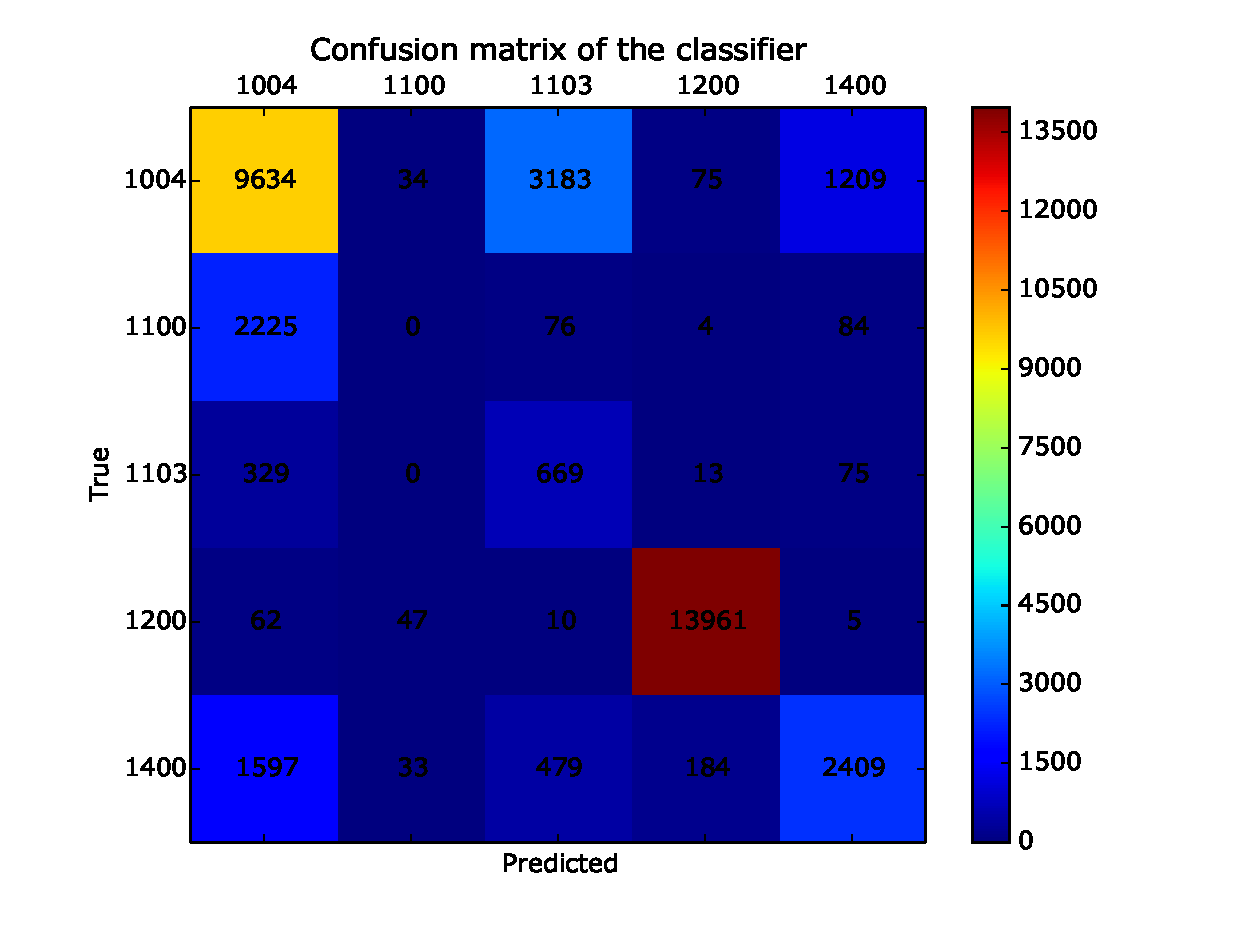
\includegraphics[scale=0.4,trim = 0.3 0.3 0.3 0.3,clip]{figs/winnow_amtoan_test1.eps}
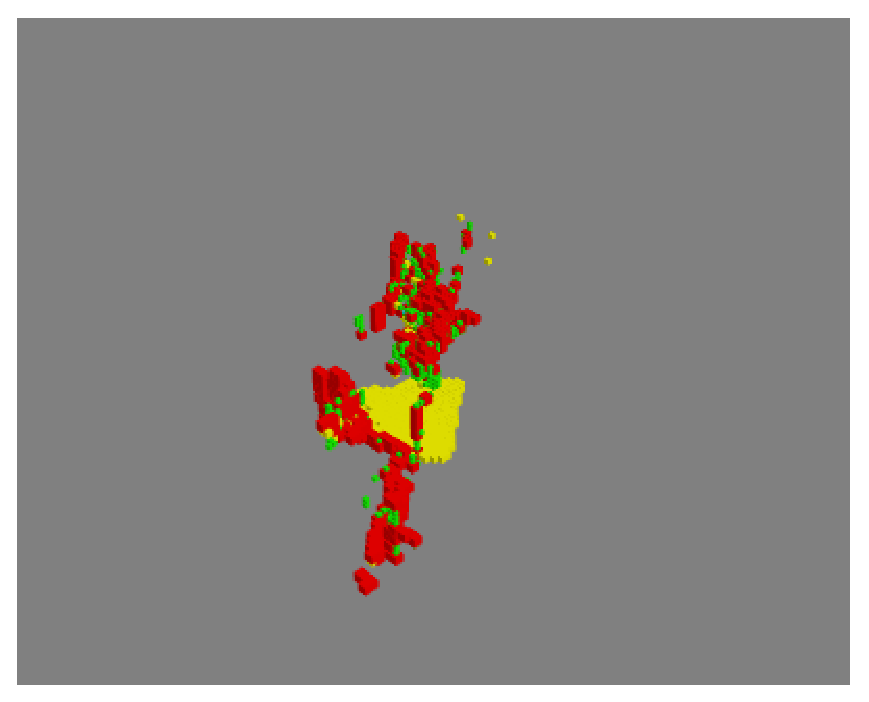
\includegraphics[scale=0.4]{figs/winnow_amtoan_test1_plot.eps}
\caption{Multiclass Winnow trained on the am dataset, testing on the an}
\vspace{0.1 in}
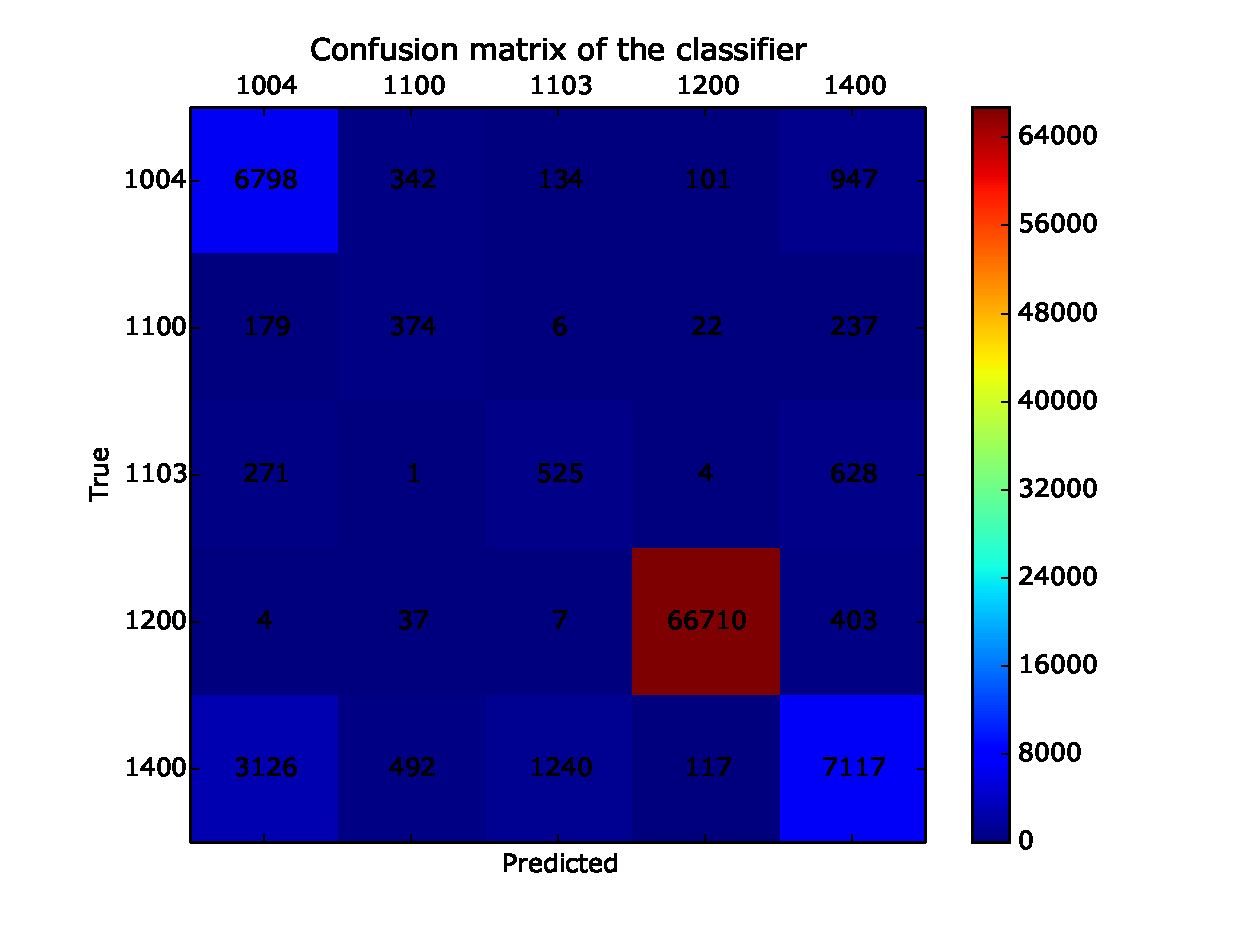
\includegraphics[scale=0.4,trim = 0.3 0.3 0.3 0.3,clip]{figs/winnow_antoam_test1.eps}
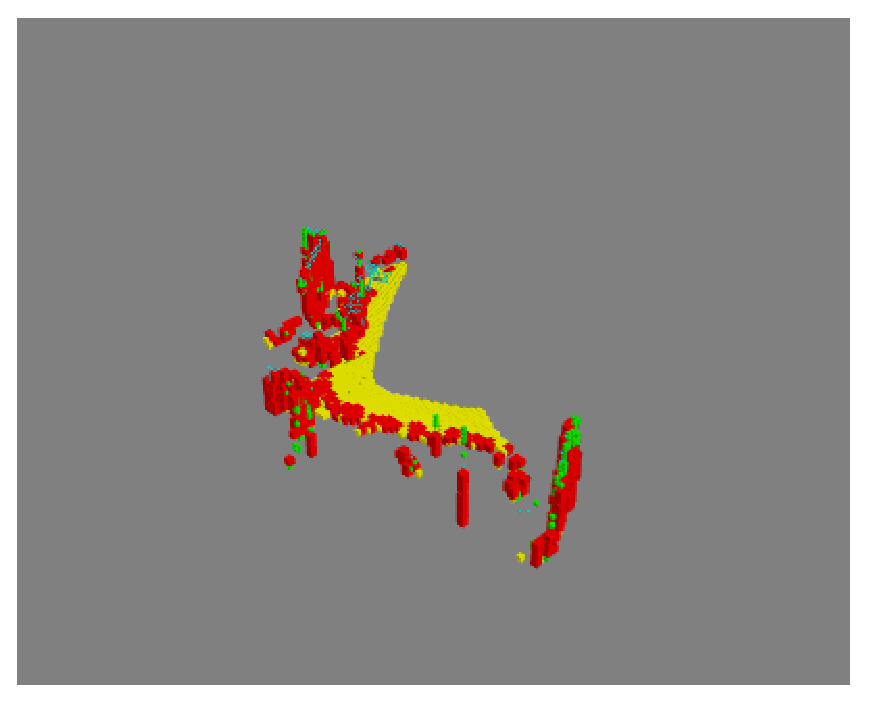
\includegraphics[scale=0.4]{figs/winnow_antoam_test1_plot.eps}
\caption{Multiclass Winnow trained on the an dataset, testing on the am}
\label{}
\end{figure}
%----------------------------------------------------------------------
\subsection{Kernalized SVM}


%-----------------------------------------------------------------------
\section{Comparative Analysis of Learners}
SVM fits the best to the data due to the advantage of the kernels.

\section{Future Work}
Augment features using spatial context, e.g., 3D HoG.\\
\end{document}